\bookchapter{Imitating motions: BeyondMimic and AMP}\label{ch:mj3}

\section*{Explanation}
Writing a reward for ``walk like a human'' is hard: stand upright, lift the feet, swing the arms, do not drag the toes, and so on, each with a weight. People solved this problem in a different way: instead of describing the motion in words, \textbf{show it}. A human moves in a motion-capture studio; the motion is converted (``retargeted'') to the joints of the robot; and the reward becomes ``be like the reference''. There are two main ways to use such a reference, and both are available for the Booster robots in the project \texttt{booster-mjlab}:
\begin{itemize}[nosep]
 \item \textbf{Motion tracking} (the family of DeepMimic and BeyondMimic): follow the \emph{exact} reference, frame by frame. You get a precise copy of one motion.
 \item \textbf{Adversarial motion priors (AMP)}: a second network, a \emph{discriminator}, judges whether the robot ``moves like the dataset''. The reference is only used as a \emph{style}; the robot is free to do a different task in that style.
\end{itemize}
As before, the descriptions in this chapter come from reading the documentation and the source code of mjlab and booster-mjlab. I did not train these tasks. The two small programs that were run are toys that show a mechanism.

\section*{Where the reference motions come from}
A reference motion is a sequence of poses: for each frame the position and orientation of the base and all joint angles. The common sources are motion-capture data sets of humans (for example LAFAN1 and AMASS). The human skeleton differs from that of the robot (other lengths, other joints), so the motion is \textbf{retargeted}: an optimisation finds the joint angles of the robot that look like the human pose; an open-source tool for this is GMR (``general motion retargeting''), which booster-mjlab names as compatible.

Two practical things matter. First, the \textbf{licence}: retargeting changes the representation, not the copyright. The repository explicitly keeps all motion files out of the code repository and explains that for example LAFAN1 is distributed under a licence (CC BY-NC-ND) that does not permit sharing adapted material, and that AMASS and its sub-data sets have their own terms. If you train a policy on such data, keep a note of the provenance of every clip. Second, the \textbf{format}: mjlab expects its own \texttt{.npz} file for tracking, produced from a CSV (base position, base quaternion, joint angles) by a converter that runs the motion through the simulator, computes the positions of all bodies, and resamples the frame rate (for example from $30$ to $50$\,Hz). The documentation warns that you \emph{must} use this converter: the file stores body positions indexed by the order of the bodies, and different physics engines order the bodies differently, so a file from another framework maps the targets to the wrong bodies, and ``training will not converge''. The AMP tasks of booster-mjlab read another format, GMR-style pickle files with the fields \texttt{dof\_pos}, \texttt{root\_pos}, \texttt{root\_rot}, positions of the key bodies and the frame rate.

\section*{Motion tracking (BeyondMimic)}
BeyondMimic (arXiv:2508.08241, ``From Motion Tracking to Versatile Humanoid Control via Guided Diffusion'') is a framework for whole-body humanoid control. As I understand it, its basis is a robust \textbf{motion-tracking policy}, trained with reinforcement learning for each motion; as the title says, diffusion is used on top of such policies for more versatile control. This chapter treats only the tracking part. The mjlab documentation refers to the instructions of the BeyondMimic project for the preparation of the motions, and its tracking task follows that set-up.

\textbf{The command} is the reference motion: at every step the environment knows which frame of the motion the robot should be in. The robot has an \textbf{anchor body} (the torso) and a list of tracked bodies.

\textbf{The observation} of the actor contains the reference command (the reference joint positions and velocities of the current frame), the pose of the reference anchor in the frame of the robot's anchor, the linear and angular velocity of the IMU sensor, the joint positions and velocities, and the last action; all with noise. The critic also gets the positions and orientations of the bodies.

\textbf{The reward} is a sum of exponential kernels, each of the form $\exp(-\text{error}^2/\sigma^2)$ (Chapter~\ref{ch:mj2}). From the configuration of mjlab:
\begin{center}
\small
\begin{tabular}{lcc}
\hline
term & weight & $\sigma$\\
\hline
position of the anchor (global) & $0.5$ & $0.3$\\
orientation of the anchor (global) & $0.5$ & $0.4$\\
positions of the bodies (relative to the anchor) & $1.0$ & $0.3$\\
orientations of the bodies (relative) & $1.0$ & $0.4$\\
linear velocities of the bodies & $1.0$ & $1.0$\\
angular velocities of the bodies & $1.0$ & $3.14$\\
action rate (penalty) & $-0.1$ & \\
joint position limits (penalty) & $-10$ & \\
self collision (penalty) & $-10$ & \\
\hline
\end{tabular}
\end{center}
The sum of the six positive terms is at most $5$ per step. Note the large penalties for self-collision and joint limits: a motion from a human can ask the robot for a pose that its legs cannot reach.

\textbf{The terminations} stop an episode early when the robot is clearly lost: when the height of the anchor differs from the reference by more than $0.25$\,m, when its orientation is off by more than a threshold, or when the height of an end effector (the feet and wrists) is off by more than $0.25$\,m. Without early termination the robot would waste experience lying on the floor while the reference keeps on dancing.

\textbf{The start of an episode} is not always the start of the motion: the robot is placed at a \emph{random phase} of the reference (``reference state initialisation''), with small random offsets. The default sampling mode of mjlab is \textbf{adaptive}: the motion is cut into time bins, the number of failures in each bin is counted (with a slowly decaying average), and the starts are drawn with a probability proportional to the failures (plus a uniform part of $10\%$), so that the robot practises the hard part, a jump, a landing, more often than the easy part.

\begin{center}
\begin{tikzpicture}[>={Stealth[length=2.2mm]},bx/.style={draw,thick,rounded corners=3pt,minimum width=2.6cm,minimum height=0.85cm,font=\scriptsize,align=center}]
 \node[bx,fill=gray!15] (mc) at (0,0) {motion capture\\ (human)};
 \node[bx,fill=gray!15] (rt) at (3.2,0) {retarget\\ (GMR)};
 \node[bx,fill=yellow!20] (cv) at (6.4,0) {convert\\ (\texttt{csv\_to\_npz})};
 \node[bx,fill=blue!10] (tr) at (9.6,0) {train\\ (tracking task)};
 \node[bx,fill=green!12] (pl) at (9.6,-1.5) {play and\\ evaluate};
 \draw[->,thick] (mc)--(rt); \draw[->,thick] (rt)--(cv); \draw[->,thick] (cv)--(tr); \draw[->,thick] (tr)--(pl);
 \node[font=\scriptsize,align=center] at (4.8,-1.5) {licence of the data!\\ keep the provenance};
\end{tikzpicture}
\captionof{figure}{The pipeline of motion tracking. The converter is part of mjlab; the registry of the documentation (Weights \& Biases) stores the converted motions. In booster-mjlab the tracking environment of the T1 reads a local file named by the variable \texttt{MJLAB\_TRACKING\_MOTION\_FILE}.}
\end{center}

\subsection*{Adaptive sampling in a toy}
The following program shows only the \emph{mechanism}. A motion has $20$ time bins; two of them are hard (failure probability $0.5$) and the others easy ($0.03$); every time a bin is practised its failure probability falls, $p\leftarrow p\,e^{-0.002\,n}$ for $n$ starts. The program counts the iterations (of $1024$ starts each) until no bin is worse than $5\%$. The numbers are my assumptions; the point is the comparison of the two sampling rules.
\begin{verbatim}
import numpy as np

BINS, N, ALPHA, UNI = 20, 1024, 0.05, 0.1

def run(adaptive, seed, max_it=400):
    rng = np.random.default_rng(seed)
    p = np.full(BINS, 0.03)
    p[12:14] = 0.5                       # a hard part of the motion
    fail_ema = np.zeros(BINS)
    for it in range(max_it):
        if p.max() < 0.05:
            return it, p.max()
        if adaptive:
            w = fail_ema + UNI / BINS
            w = w / w.sum()
        else:
            w = np.full(BINS, 1.0 / BINS)
        n = rng.multinomial(N, w)        # starts per bin
        f = rng.binomial(n, p)           # failures per bin
        fail_ema = ALPHA * f + (1 - ALPHA) * fail_ema
        p = p * np.exp(-0.002 * n)       # practice makes better
    return max_it, p.max()

for mode in (False, True):
    its = [run(mode, s)[0] for s in range(100)]
    print("adaptive" if mode else "uniform ", "median iterations:",
          int(np.median(its)), " 90th percentile:",
          int(np.percentile(its, 90)))
\end{verbatim}
In $100$ runs the uniform sampling needed a median of $23$ iterations ($90\%$ of the runs: $24$) and the adaptive sampling a median of $4$ ($90\%$: $5$). In the real task the effect is smaller and noisier, but this is why a long motion with one difficult part, a kick, can be learned at all.

\section*{Adversarial motion priors (AMP)}
Tracking has a weakness for soccer. A kick that is tracked exactly is a kick of the \emph{reference}: the ball must be where the reference had it, and the robot must start from the reference posture. A robot that has to walk to \emph{any} goal position and turn to \emph{any} angle cannot use a single reference clip.

AMP (Peng et al., 2021, arXiv:2104.02180) solves this by learning the reward from the data. A \textbf{discriminator} $D$ receives a pair of consecutive states $(s,s')$ and has to decide whether it came from the dataset (``expert'') or from the policy. The policy gets a \textbf{style reward} that is high when it fools the discriminator, and a \textbf{task reward} for what you actually want (reach the goal). Unlike tracking, there is no time index and no phase: the data can be many unrelated clips, and the robot may combine them.

\begin{center}
\begin{tikzpicture}[>={Stealth[length=2.2mm]},bx/.style={draw,thick,rounded corners=3pt,minimum width=2.5cm,minimum height=0.85cm,font=\scriptsize,align=center}]
 \node[bx,fill=gray!15] (ds) at (0,1.4) {reference clips\\ (walk, run, sprint)};
 \node[bx,fill=blue!10] (pol) at (0,-1.4) {policy in the\\ simulator};
 \node[bx,fill=orange!15] (dis) at (4.2,0) {discriminator\\ $D(s,s')$};
 \node[bx,fill=green!12] (rs) at (8,0.9) {style reward};
 \node[bx,fill=yellow!20] (rt) at (8,-0.9) {task reward\\ (reach the goal)};
 \node[bx,fill=red!10] (mix) at (11.2,0) {mix, PPO\\ update};
 \draw[->,thick] (ds)--node[above left,font=\scriptsize]{label 1} (dis);
 \draw[->,thick] (pol)--node[below left,font=\scriptsize]{label $-1$} (dis);
 \draw[->,thick] (dis)--(rs); \draw[->,thick] (pol.east) to[out=0,in=180] (rt.west);
 \draw[->,thick] (rs)--(mix); \draw[->,thick] (rt)--(mix);
 \draw[->,thick,dashed] (mix.south) to[out=-90,in=-60,looseness=0.8] node[below,font=\scriptsize]{better policy} (pol.south east);
\end{tikzpicture}
\captionof{figure}{AMP. The discriminator is trained to separate reference transitions from the transitions of the policy; the policy is trained with PPO on a mixture of a style reward (from the discriminator) and a task reward.}
\end{center}

\subsection*{AMP in booster-mjlab}
The shared AMP code of the repository has a discriminator, a replay buffer of policy transitions, a motion loader, and a PPO variant that adds the style reward. The numbers below are those of the K1 configuration.

\textbf{State.} The discriminator does not see the command or the goal, only a description of how the robot \emph{moves}: for the K1 with $22$ joints it is $22$ joint positions, $22$ joint velocities, the height of the base ($1$), the projected gravity ($3$), the linear and angular velocity of the base in its own frame ($3+3$), and the positions and velocities of four \emph{key bodies} (both hands and both feet) relative to the base ($12+12$): in total $78$ numbers. The discriminator takes two consecutive states, $156$ inputs, through a network with layers of $512$ and $256$ units, normalised inputs.

\textbf{Loss.} In the configuration of the K1 the loss is the least-squares one: the target of $D$ is $+1$ for reference transitions and $-1$ for policy transitions,
\[
L_D=\tfrac12\Big(\mathbb E_{\text{ref}}\big[(D-1)^2\big]+\mathbb E_{\text{policy}}\big[(D+1)^2\big]\Big)+10\;\mathbb E_{\text{ref}}\big[\|\nabla D\|^2\big],
\]
where the last term is a \textbf{gradient penalty} (coefficient $10$) that keeps the discriminator smooth, so that its reward does not jump. The learning rate of the discriminator is $3\cdot10^{-4}$; the replay buffer holds $100\,000$ transitions.

\textbf{Style reward.} For the least-squares loss the score is
\[
r_{\text{style}}=\max\!\big(0,\;1-\tfrac14(D-1)^2\big),
\]
which is $1$ for $D=1$ (as good as the reference), $0.75$ for $D=0$, and $0$ for $D\le-1$ (clearly policy-like). The code has other score functions (a sigmoid, and a ``softplus'' one that is normalised and clipped at $1.5$).

\begin{center}
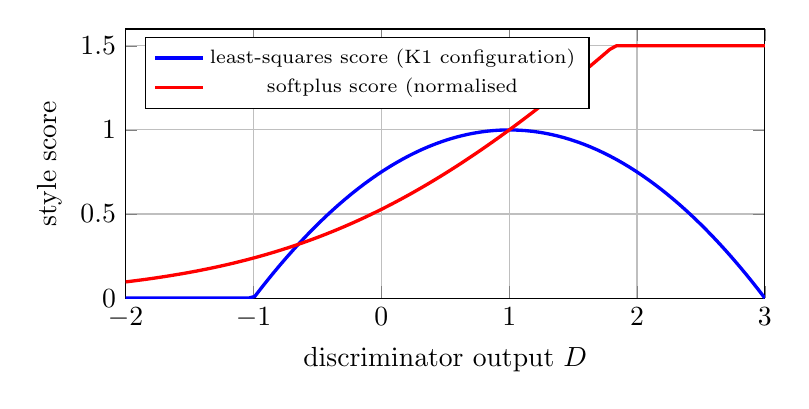
\begin{tikzpicture}
\begin{axis}[width=0.8\linewidth,height=5cm,xlabel={discriminator output $D$},ylabel={style score},xmin=-2,xmax=3,ymin=0,ymax=1.6,grid=both,samples=100,legend style={font=\scriptsize,at={(0.03,0.97)},anchor=north west}]
 \addplot[blue,very thick,domain=-2:3] {max(0,1-0.25*(x-1)^2)};
 \addplot[red,very thick,domain=-2:3] {min(1.5, ln(1+exp(x))/1.3133)};
 \legend{least-squares score (K1 configuration),softplus score (normalised, clipped at 1.5)}
\end{axis}
\end{tikzpicture}
\captionof{figure}{Two of the score functions of the discriminator code. The blue one is bounded by $1$, falls to $0$ for policy-like transitions, and is the one used by the K1 configuration; the red one keeps rising for large $D$ (up to the clip at $1.5$).}
\end{center}

\textbf{Mixing.} The reward that PPO sees is
\[
r=(1-\lambda)\,c\,r_{\text{style}}+\lambda\,r_{\text{task}},
\]
with the scale $c=0.6$ and $\lambda=0.45$ in the K1 configuration.

\begin{example}
The discriminator gives $D=0.5$ for a transition. The style score is $1-\tfrac14(0.5-1)^2=0.9375$, scaled $0.6\cdot0.9375=0.5625$. The task reward of this step is $0.2$. Then $r=0.55\cdot0.5625+0.45\cdot0.2=0.309+0.090=0.40$. A policy that stands still has a task reward of $0$ and a low style score as soon as the discriminator sees that no reference clip stands like this; a policy that runs to the goal in an unnatural way gets the task reward but a low style reward.
\end{example}

\textbf{The task.} \verb!Mjlab-TargetLocationAmp-Flat-Booster-K1!: the command is a \textbf{goal pose} (a position and a yaw angle relative to the robot); the robot has to reach it and stand there. The episode is $6$\,s; it ends with success when the robot has been within $0.16$\,m and $0.20$\,rad of the goal for $25$ steps, with a speed below $0.35$\,m/s, a turning rate below $0.6$\,rad/s and the trunk nearly upright. The rewards include a progress reward for the reduction of the distance and the yaw error, a bonus for reaching the goal, penalties for the action rate, the joint limits and the roll and pitch rates, a reward for the base height and the upright trunk, and a reward for time efficiency. A \textbf{goal curriculum} grows the distance of the goals in four stages: $0.4$--$1.2$\,m at the start, then up to $2.4$, $4.0$ and finally $6.0$\,m, with the full yaw range in the last stage. The reference data are the walk, run and sprint clips of the LAFAN1 set retargeted to the K1 (which you must prepare yourself; they are not distributed). The learning part uses PPO with the clip parameter $0.2$, learning rate $10^{-3}$ with the adaptive KL schedule (target $0.01$), discount $0.98$, $\lambda_{\text{GAE}}=0.95$, $5$ epochs and $4$ mini-batches, $24$ steps per environment and iteration, $1024$ environments, a network of $512$-$256$-$128$ units with ELU, an initial action standard deviation of $0.45$ and up to $10\,000$ iterations.

\begin{keyidea}[Tracking or AMP?]
\begin{center}
\small
\begin{tabular}{p{2.6cm}p{5cm}p{5cm}}
\hline
 & motion tracking & AMP\\
\hline
reference used as & exact target, frame by frame & style: ``be like the data''\\
needs a command & no (the clip is the command) & yes (goal, velocity), plus a task reward\\
data & one clip per policy & many clips, may be unrelated\\
result & a precise copy of one motion & a flexible controller in the style\\
risk & only works near the reference & the discriminator can be fooled; training can be unstable\\
good for & a kick, a get-up, a dance & walking to any place\\
\hline
\end{tabular}
\end{center}
\end{keyidea}

\begin{aibox}[Imitation and the real robot]
The reference motion is made for a human body. Before it goes to hardware, check at least: do the joint angles lie inside the real limits? Are the velocities and torques below what the motors can do? Does the foot contact make sense (no skating)? A policy trained on an impossible motion learns to \emph{fail gracefully in the simulator} and fails on the robot.
\end{aibox}

\section*{Practice problems}
\begin{enumerate}[label=\textbf{\thechapter.\arabic*}]
  \item Compute the six tracking terms for an anchor position error of $0.1$\,m (with $\sigma=0.3$), an orientation error of $0.2$\,rad ($\sigma=0.4$) and a mean body-position error of $0.05$\,m ($\sigma=0.3$). What is the weighted sum of these three terms (weights $0.5$, $0.5$, $1.0$)?
  \item A tracking policy is perfect except for the global position of the anchor: it is $0.5$\,m off. Which of the terms of the table fall, and which stay at $1$? What does this say about the design with a global and a relative term?
  \item Explain why a termination condition on the height of the feet is useful. What happens to the learning signal if there is no termination and the robot falls at second $2$ of a $10$\,s motion?
  \item A motion lasts $12$\,s at $50$\,Hz. How many frames? It is cut into $20$ bins: how many frames per bin? Which bin contains the time $7.3$\,s?
  \item Give the style score $\max(0,1-\tfrac14(D-1)^2)$ for $D=-1,0,0.5,1,2$. Why is the score not larger than $1$?
  \item With $c=0.6$, $\lambda=0.45$: compute the reward $r$ for (a) $D=1$, $r_{\text{task}}=0$; (b) $D=-1$, $r_{\text{task}}=1$; (c) $D=0$, $r_{\text{task}}=0.5$. Which behaviour does the mixture prefer, (a) or (b)?
  \item Count the dimension of the AMP state for a robot with $23$ joints and $4$ key bodies, and of the input of the discriminator. Check the number $78$ for the K1.
  \item A discriminator is much too strong: it separates policy and data perfectly ($D=-1$ for the policy). What is the style reward, what does the policy gradient look like, and what does the gradient penalty do about it?
  \item Why can AMP use many unrelated clips, but tracking needs one? What happens if the data set contains only forward walking, and the task asks for a turn on the spot?
  \item[\textbf{\thechapter.10}$\star$] Change the adaptive-sampling toy so that the failure rate depends on a neighbouring bin as well (a failure at bin $12$ makes bin $11$ twice as likely to fail), and add the smoothing kernel of the code (a convolution of the sampling probabilities with a short kernel). Report the median iterations for uniform and adaptive sampling.
\end{enumerate}

\section*{Further reading}
\begin{itemize}[nosep]
 \item K.~Zakka et al., \emph{mjlab: A Lightweight Framework for GPU-Accelerated Robot Learning}, arXiv:2601.22074.
 \item X.~B.~Peng, Z.~Ma, P.~Abbeel, S.~Levine, A.~Kanazawa, \emph{AMP: Adversarial Motion Priors for Stylized Physics-Based Character Control}, 2021, arXiv:2104.02180.
 \item \emph{BeyondMimic: From Motion Tracking to Versatile Humanoid Control via Guided Diffusion}, arXiv:2508.08241.
\end{itemize}
